\documentclass[12pt]{IEEEtran}
%\IEEEoverridecommandlockouts
\usepackage{cite}
\usepackage{url}
\usepackage{amsmath,amssymb,amsfonts}
\usepackage{algorithmic}
\usepackage{graphicx}
\usepackage{textcomp}
\usepackage{xcolor}
\usepackage{array}
\usepackage{tikz}
\usetikzlibrary{positioning,arrows.meta}
\def\BibTeX{{\rm B\kern-.05em{\sc i\kern-.025em b}\kern-.08em
 T\kern-.1667em\lower.7ex\hbox{E}\kern-.125emX}}

% Draft helper: visible TODO notes. Remove before final submission.
\newcommand{\todo}[1]{\textcolor{red}{[TODO: #1]}}

\begin{document}

\title{Cross-Domain Evaluation of LLM-Assisted Secure Code Generation: Preserving Safety Properties in Automotive and Avionics Firmware}

\author{
\IEEEauthorblockN{Evan C Hardt, The University of Alabama}\\
\IEEEauthorblockN{Benjamin S Swartley, The University of Alabama}%
}
\maketitle

% =====================================================================
\begin{abstract}
Large language models (LLMs) are increasingly used to generate and repair source code, including firmware for safety-critical transportation systems. Recent work argues that secure code generation techniques must be evaluated on both security and functionality, since a technique that removes a reported weakness can also break the program it was meant to protect. Embedded transportation software, however, carries a third requirement that functional tests do not capture: compliance with safety coding standards such as MISRA-C, which prohibit constructs like dynamic memory allocation and recursion and require bounded, deterministic control flow. A security patch can pass every functional test and still violate these constraints. This paper proposes an empirical study of whether LLM-assisted secure code generation and repair preserves safety-coding-rule compliance, and whether the resulting security/safety tradeoff is consistent across two structurally different transportation protocol domains: ASCII-text CAN frame parsing in the automotive \texttt{can-utils} library and binary Mode~S/ADS-B decoding in the avionics \texttt{dump1090} decoder. We seed seven known weaknesses (CWE-20, CWE-120/787, CWE-125, and CWE-190) into these codebases and apply three techniques: baseline prompting, security-focused prompting, and static-analysis-guided repair. Each generated patch is evaluated along three axes: security (Cppcheck and Semgrep), safety (a fixed MISRA-C:2012 rule subset), and functionality (unit tests). We plan to report CWE-fix rate, safety-violation-introduction rate, functional pass rate, security/safety tool disagreement, and per-domain variance.
\end{abstract}

\begin{IEEEkeywords}
large language models, secure code generation, automated program repair, MISRA-C, embedded systems, automotive security, avionics security, CAN bus, ADS-B
\end{IEEEkeywords}

% =====================================================================
\section{Introduction}
\IEEEPARstart{L}{arge} language models are now a routine part of software development, and their use is spreading into embedded and safety-critical domains. Developers use code assistants to write new functions, explain unfamiliar code, and increasingly to repair security defects flagged by static analyzers. At the same time, a growing body of work shows that LLM-generated code frequently contains security weaknesses~\cite{pearce2022asleep, khoury2023chatgpt, tihanyi2023formai}, and that developers who rely on AI assistants may produce less secure code while believing it to be more secure~\cite{perry2023users}. In response, researchers have proposed techniques to make generated code more secure, including security-focused prompting, controlled generation~\cite{he2023sven}, and LLM-driven vulnerability repair~\cite{pearce2023zeroshot}.

Evaluating these techniques is harder than it looks. Dai et al.~\cite{rethinking2026} show that a technique can lower the number of reported security warnings while damaging the program: it may delete the vulnerable code path entirely, return early without doing the required work, or replace the original logic with code that no longer solves the task. They argue that security and functionality must therefore be evaluated together on the same generated programs.

We argue that, for embedded transportation software, two axes are still not enough. Automotive and avionics firmware is commonly written against safety coding standards such as MISRA-C~\cite{misra2012}, and avionics software is developed under certification processes such as DO-178C~\cite{do178c}. These standards restrict constructs that make code hard to analyze or bound: heap allocation, recursion, unbounded loops, and multiple exit points. The constructs an LLM reaches for when ``making code safe'' in a general-purpose sense, such as allocating a right-sized buffer with \texttt{malloc}, adding several early \texttt{return} statements for each error case, or wrapping parsing in a retry loop, are exactly the constructs these standards discourage. A patch that removes a buffer overflow and passes every functional test can still be unacceptable in a vehicle or an aircraft. Standard security-plus-functionality evaluation would score that patch as a success.

A second, related question is whether this tradeoff is a property of the technique or of the code it is applied to. Transportation software spans very different input representations. Automotive tooling built around SocketCAN often parses human-readable ASCII representations of CAN frames, while avionics receivers such as ADS-B decoders operate on raw binary messages with bit-level field extraction and arithmetic-heavy position decoding. These representations expose different weakness classes (string handling and length validation versus bit indexing and integer arithmetic) and may draw out different LLM repair behaviors.

This paper proposes an empirical study that addresses both questions. We seed seven weaknesses into two open-source transportation codebases, \texttt{can-utils}~\cite{canutils} and \texttt{dump1090}~\cite{dump1090}, apply three LLM-assisted generation and repair techniques, and evaluate every resulting patch for security, safety-rule compliance, and functional correctness. We then compare the results across the two domains.

The planned contributions of this work are:
\begin{itemize}
    \item A three-axis evaluation (security, safety, functionality) of LLM-assisted secure code repair for embedded C, extending the dual-axis evaluation of Dai et al.~\cite{rethinking2026}.
    \item A small, reproducible benchmark of seeded weaknesses in real automotive and avionics code, with a fixed, explicitly defined MISRA-C rule subset as an operational safety criterion.
    \item A measurement of how often security scanners and safety-rule checkers disagree about the same patch.
    \item A cross-domain comparison of whether the security/safety tradeoff differs between text-based and binary protocol code.
\end{itemize}

% =====================================================================
\section{Problem Statement}
LLM-driven security repair can remove a CWE from embedded C code while introducing violations of safety-critical coding constraints, such as dynamic memory allocation, recursion, unbounded loops, or multiple function exit points. Current evaluation practice for secure code generation checks whether a patch removes the weakness and whether it still passes functional tests~\cite{rethinking2026}, but neither check detects safety-rule regressions. As a result, a technique that looks effective under existing benchmarks may produce code that cannot be deployed in a safety-critical system.

This risk may also depend on the protocol representation being processed. ASCII-text parsing, as in CAN frame parsing in \texttt{can-utils}, and binary bit-level decoding, as in Mode~S/ADS-B decoding in \texttt{dump1090}, present different CWE surfaces and may lead to different LLM failure modes. If the security/safety tradeoff varies by domain, conclusions drawn from one kind of embedded code will not transfer to another, and evaluations built on a single domain will give a misleading picture of a technique's reliability.

The problem matters for software engineering practice because LLM-based repair is being adopted faster than the evaluation methods that would tell practitioners whether its output is acceptable in regulated domains. It matters for research because it identifies a dimension, safety-standard compliance, that is missing from current secure-code-generation benchmarks.

% =====================================================================
\section{Preliminary Research Questions}
This study is organized around three preliminary research questions. We expect to refine them after pilot runs.

\textbf{RQ1: Does an LLM-generated security fix for a CWE in embedded C preserve compliance with safety coding rules?}
For each seeded weakness and technique, we measure whether the patch removes the weakness and whether it introduces new violations of a fixed MISRA-C:2012 rule subset relative to the pre-patch code.

\textbf{RQ2: Do security scanners and safety-rule checkers disagree about the same patched code?}
We measure how often a patch is judged acceptable by the security tools but not by the safety checker, and the reverse, and characterize the kinds of code changes that produce disagreement.

\textbf{RQ3: Does the security/safety tradeoff generalize across protocol domains?}
We compute the RQ1 and RQ2 metrics separately for the text-based automotive tasks (\texttt{can-utils}) and the binary avionics tasks (\texttt{dump1090}) and compare them for consistency or divergence.

% =====================================================================
\section{Related Work}

\subsection{Security of LLM-Generated Code}
Pearce et al.~\cite{pearce2022asleep} evaluated GitHub Copilot on scenarios built around MITRE's top CWEs and found that roughly 40\% of the generated programs contained vulnerabilities. Follow-up studies reported similar results for ChatGPT~\cite{khoury2023chatgpt} and, at much larger scale, for C programs generated by GPT-3.5 and verified with bounded model checking in the FormAI dataset~\cite{tihanyi2023formai}. Perry et al.~\cite{perry2023users} conducted a user study showing that participants with access to an AI assistant wrote less secure code and were more confident in its security. These studies establish that LLM output cannot be assumed secure, but they evaluate general-purpose code and do not consider safety-coding constraints.

\subsection{Techniques for Secure Generation and Repair}
Several techniques aim to improve the security of LLM output. He and Vechev~\cite{he2023sven} proposed SVEN, which uses learned continuous prefixes to steer a code model toward secure outputs without changing its weights. Pearce et al.~\cite{pearce2023zeroshot} studied zero-shot vulnerability repair, showing that LLMs can fix many synthetic and real-world vulnerabilities when prompted appropriately, but that results are sensitive to prompt wording and context. Static-analysis feedback loops, in which analyzer warnings are fed back into the prompt, are a common pattern in this space. Our three techniques (baseline prompting, security-focused prompting, and static-analysis-guided repair) are chosen to represent the low-cost, prompt-level end of this spectrum, which is the most likely to be adopted by practitioners without model access.

\subsection{Evaluating Secure Code Generation}
Dai et al.~\cite{rethinking2026} argue that prior evaluations overstate the effectiveness of secure code generation techniques because they measure security in isolation. They show that techniques can reduce reported weaknesses by removing or degrading required functionality, and they call for joint evaluation of security and functionality on the same generated programs. They also raise the question of whether a technique's effectiveness transfers across programming languages. Our study adopts their joint-evaluation principle, adds safety-standard compliance as a third axis, and reframes their generalization question in terms of protocol representation rather than programming language.

\subsection{Static Analyzer Agreement}
Lipp et al.~\cite{lipp2022static} evaluated several static C analyzers against real-world vulnerabilities and found that individual tools miss a large fraction of vulnerabilities and that their results vary considerably. This motivates RQ2: if security analyzers disagree among themselves, we should not expect a security analyzer and a safety-rule checker, which are built for different goals, to agree about whether a patch is acceptable.

\subsection{Safety Coding Standards}
MISRA-C~\cite{misra2012} provides guidelines for writing C in critical systems. It restricts constructs that are difficult to verify or bound, including dynamic memory allocation, recursion, and multiple exit points from a function. DO-178C~\cite{do178c} defines the software life-cycle and assurance processes required for airborne software certification. This project does not claim compliance with either standard. Instead, it uses a small, checkable subset of MISRA-C rules as an operational definition of ``safety-preserving'' code.

\subsection{Transportation Protocol Security}
Both target domains have well-documented security problems at the protocol level. Koscher et al.~\cite{koscher2010experimental} demonstrated that an attacker with access to a vehicle's CAN bus could control safety-critical functions, because the bus provides no authentication and electronic control units (ECUs) trust incoming frames. Strohmeier et al.~\cite{strohmeier2015adsb} surveyed the security of ADS-B, which broadcasts unauthenticated, unencrypted position reports that any receiver can decode and any transmitter can spoof. In both domains, the parsing and decoding code that handles untrusted input sits directly on the attack surface, which makes it a realistic and relevant target for security repair.

\subsection{The Gap}
To our knowledge, no existing work evaluates LLM-driven security repair against safety-coding constraints, and no work examines whether such a tradeoff, if it exists, is consistent across differently structured protocol domains. This project addresses both gaps by pairing a security-focused evaluation pipeline with a safety-rule checker and applying the same pipeline to two transportation codebases from different domains. Related work on LLMs for embedded and firmware code, and on static-analysis-guided LLM repair, will be expanded in the next milestone.

% =====================================================================
\section{Proposed Methodology}
This is an empirical study. Fig.~\ref{fig:pipeline} summarizes the pipeline: each seeded task is given to each technique and model, and every resulting patch is evaluated by the same three-axis harness.

\begin{figure}[t]
\centering
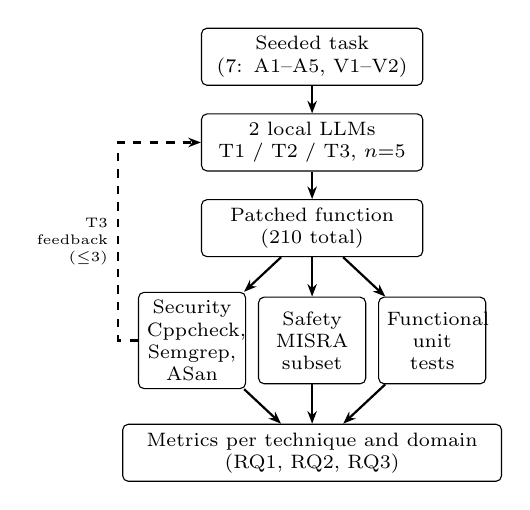
\begin{tikzpicture}[
    node distance=0.35cm and 0.3cm,
    box/.style={draw, rounded corners=2pt, align=center, font=\scriptsize, minimum height=0.6cm, inner sep=3pt},
    arr/.style={-{Stealth[length=1.6mm]}, thick}
]
\node[box, text width=2.6cm] (task) {Seeded task\\(7: A1--A5, V1--V2)};
\node[box, text width=2.6cm, below=of task] (llm) {2 local LLMs\\T1 / T2 / T3, $n{=}5$};
\node[box, text width=2.6cm, below=of llm] (patch) {Patched function\\(210 total)};
\node[box, text width=1.15cm, minimum height=1.1cm, below=0.5cm of patch] (saf) {Safety\\MISRA\\subset};
\node[box, text width=1.15cm, minimum height=1.1cm, left=0.15cm of saf] (sec) {Security\\Cppcheck,\\Semgrep, ASan};
\node[box, text width=1.15cm, minimum height=1.1cm, right=0.15cm of saf] (fun) {Functional\\unit tests};
\node[box, text width=4.6cm, below=0.5cm of saf] (met) {Metrics per technique and domain\\(RQ1, RQ2, RQ3)};
\draw[arr] (task) -- (llm);
\draw[arr] (llm) -- (patch);
\draw[arr] (patch) -- (sec);
\draw[arr] (patch) -- (saf);
\draw[arr] (patch) -- (fun);
\draw[arr] (sec) -- (met);
\draw[arr] (saf) -- (met);
\draw[arr] (fun) -- (met);
\draw[arr, dashed] (sec.west) -- ++(-0.25,0) |- node[pos=0.25, left, font=\tiny, align=right]{T3\\feedback\\($\leq$3)} (llm.west);
\end{tikzpicture}
\caption{Evaluation pipeline. Every patch is checked on all three axes by one shared harness; T3 feeds security warnings back to the model for up to three rounds.}
\label{fig:pipeline}
\end{figure}

\subsection{Subject Codebases}
We select two actively maintained, open-source transportation codebases with permissive or GPL-compatible licenses:
\begin{itemize}
    \item \textbf{Automotive:} \texttt{linux-can/can-utils}~\cite{canutils}, specifically \texttt{lib.c}, the shared library that parses and formats CAN, CAN~FD, and CAN~XL frames from their ASCII representation for the SocketCAN userspace tools.
    \item \textbf{Avionics:} \texttt{flightaware/dump1090}~\cite{dump1090}, a Mode~S/ADS-B decoder for aircraft transponder messages, specifically the message decoding in \texttt{mode\_s.c} and the Compact Position Reporting (CPR) decoding in \texttt{cpr.c}.
\end{itemize}
These codebases were chosen because they process untrusted input from transportation networks, are written in C, are small enough to build and test in isolation, and represent the two contrasting input representations (text and binary) that RQ3 compares.

\subsection{Seeded Tasks}
To obtain a known ground truth, we create vulnerable variants of selected functions by removing or weakening existing defensive checks. Each variant introduces a single, documented weakness. Table~\ref{tab:tasks} lists the seven planned tasks. Seeding by removing upstream checks has two advantages: the original code provides a reference fix for comparison, and the weakness is confirmed to be reachable from the function's normal inputs.

\begin{table*}[t]
    \centering
    \caption{Planned seeded tasks by codebase, function, weakness, and domain. All seeds are synthetic except A5, which is historical.}
    \label{tab:tasks}
    \begin{tabular}{|c|l|p{5.4cm}|p{4.0cm}|l|}
        \hline
        \textbf{ID} & \textbf{Codebase} & \textbf{Function (modification)} & \textbf{Seeded CWE} & \textbf{Domain} \\
        \hline
        A1 & can-utils & \texttt{hexstring2data} (length check removed) & CWE-120 / CWE-787 (buffer overflow) & Automotive \\
        \hline
        A2 & can-utils & \texttt{hexstring2data} (odd-length check removed) & CWE-20 (improper input validation) & Automotive \\
        \hline
        A3 & can-utils & \texttt{parse\_canframe} (bounds re-check removed in FD/XL branch) & CWE-125 (out-of-bounds read) & Automotive \\
        \hline
        A4 & can-utils & \texttt{can\_fd\_dlc2len} (nibble mask removed) & CWE-125 (array index) & Automotive \\
        \hline
        A5 & can-utils & \texttt{snprintf\_error\_data} (pre-fix variant reverting upstream bounds-check patch) & CWE-787 (buffer overflow) & Automotive \\
        \hline
        V1 & dump1090 & \texttt{mode\_s.c} message decode (length/type validation removed) & CWE-125 (out-of-bounds read) & Avionics \\
        \hline
        V2 & dump1090 & \texttt{cpr.c} position decode (bounds check on arithmetic removed) & CWE-190 (integer overflow) & Avionics \\
        \hline
    \end{tabular}
\end{table*}

The current task set is weighted toward the automotive domain (five tasks versus two). Before the next milestone we will search the \texttt{dump1090} commit history for real bounds and length fixes that can serve as additional historical seeds. If a balanced split cannot be reached, cross-domain comparisons will use per-task rates rather than pooled totals, and the imbalance will be reported as a limitation.

\subsection{Seeding Procedure}
Both repositories are pinned to a single tagged version (\texttt{can-utils} v2025.01 and \texttt{dump1090} v10.2), and every task is built from that baseline. We use two kinds of seeds. \emph{Synthetic} seeds remove or weaken one existing defensive check in the pinned code. \emph{Historical} seeds reverse-apply only the relevant hunk of a real upstream fix commit onto the pinned baseline, rather than checking out the full older tree, so that the only difference from the baseline is the weakness itself. Each seed is stored as a patch file in a shared repository so that any task can be rebuilt from the pinned tag. Each task also includes at least one triggering input that produces a fault under AddressSanitizer and UBSan on the seeded variant but not on the original; this input serves as ground truth for the weakness and is reused as a security regression test after repair. Results are reported separately for synthetic and historical seeds.

\subsection{Generation and Repair Techniques}
Each task is presented to the LLM as the vulnerable function plus the minimal surrounding context (type definitions, macros, and callee signatures) needed to understand it. We apply three techniques:
\begin{enumerate}
    \item \textbf{Baseline prompting (T1):} the model is asked to review and correct the function, with no mention of security.
    \item \textbf{Security-focused prompting (T2):} the model is told the function processes untrusted input and is asked to fix any security vulnerabilities.
    \item \textbf{Static-analysis-guided repair (T3):} the model receives the function together with the Cppcheck and Semgrep warnings for it and is asked to fix the reported issues. If warnings remain, the updated warnings are returned to the model for up to three rounds.
\end{enumerate}
None of the prompts mention MISRA-C or safety rules. This is deliberate: the study measures whether safety compliance is preserved \emph{incidentally}, which reflects how a developer would typically use a code assistant for a security fix. A safety-aware prompt variant may be added as an exploratory fourth condition if time permits.

\subsection{Models and Experimental Design}
All inference runs locally on a single NVIDIA RTX 4090 (24\,GB VRAM). We use two open-weight, instruction-tuned code models from different model families: Qwen2.5-Coder-32B-Instruct~\cite{qwen25coder} and Codestral-22B~\cite{codestral}, both quantized to 4-bit (GGUF \texttt{Q4\_K\_M}) and served with llama.cpp~\cite{llamacpp}. Generation uses a 16k-token context window, temperature 0.2, and a fixed, recorded random seed for each repetition; checkpoint hashes and the llama.cpp build are recorded so that every patch can be regenerated.

Each task--technique pair is repeated $n=5$ times per model to account for sampling variability. With seven tasks, three techniques, five repetitions, and two models, the design yields 210 patches.

\subsection{Evaluation Harness}
Every patch is evaluated on three axes using one shared harness, built before either codebase's tasks are run so that results are directly comparable.

\textbf{Security.} We run Cppcheck and Semgrep (with CWE-relevant C rules) on the patched function and confirm results manually against the known seeded weakness. A patch is counted as \emph{fixing} the CWE if the seeded weakness is no longer present on manual review and no new security warnings are introduced.

\textbf{Safety.} We check a fixed subset of MISRA-C:2012 rules, run primarily through Cppcheck's MISRA addon:
\begin{itemize}
    \item No dynamic memory allocation (Rule 21.3).
    \item No direct or indirect recursion (Rule 17.2).
    \item Single point of exit (Rule 15.5).
    \item Well-formed, bounded loops (Rule 14.2 for \texttt{for} loops).
\end{itemize}
Rule 14.2 covers only \texttt{for} loops, so we will supplement it with a custom Semgrep rule or manual inspection for \texttt{while} and \texttt{do} loops whose termination does not depend on a fixed bound. Because the original upstream code may not be fully compliant with this subset, we measure violations \emph{introduced} by a patch (the difference between the patched and pre-patch function) rather than absolute compliance.

\textbf{Functionality.} We run existing unit tests where available and write task-specific tests otherwise, covering valid frames and messages, boundary-length inputs, and malformed inputs. A patch passes if it compiles and passes all tests, including tests confirming that valid inputs produce the same output as the original upstream function.

\subsection{Metrics and Analysis}
For each task, technique, and domain we compute:
\begin{itemize}
    \item \textbf{CWE-fix rate:} fraction of patches that remove the seeded weakness.
    \item \textbf{Safety-violation-introduction rate:} fraction of patches that introduce at least one new violation of the rule subset.
    \item \textbf{Functional pass rate:} fraction of patches that compile and pass all tests.
    \item \textbf{Joint success rate:} fraction of patches that are secure, safe, and functional at once.
    \item \textbf{Tool disagreement rate:} fraction of patches judged acceptable by the security tools but not by the safety checker, or the reverse (RQ2).
    \item \textbf{Per-domain variance:} differences in the above between the automotive and avionics task sets (RQ3).
\end{itemize}
RQ1 is answered by comparing CWE-fix rate with safety-violation-introduction rate per technique. RQ2 is answered with the disagreement rate and a qualitative coding of the code changes behind disagreements (e.g., added \texttt{malloc}, added early returns, added retry loops). RQ3 is answered by comparing metrics between domains. Given the small number of tasks, we expect to report descriptive statistics and a qualitative comparison; a statistical test such as Fisher's exact test on per-domain pass/fail counts will be reported where sample sizes allow, with the limited power stated explicitly.

\subsection{Threats to Validity}
\textbf{Data contamination.} Both codebases are public, and the models may have seen the upstream (fixed) versions during training. A model that reproduces the upstream check from memory may look more capable than it is. We will compare patches against the upstream code to identify verbatim reproduction and report it, and we report synthetic and historical seeds separately.
\textbf{Model generalizability.} Restricting the study to 4-bit open-weight models that fit in 24\,GB means results may not transfer to larger or proprietary frontier models. In exchange, the weights are fixed and cannot change between runs, as hosted API models can.
\textbf{Tool coverage.} Free MISRA checkers cover only part of the standard. We mitigate this by fixing and reporting the rule subset in advance rather than claiming compliance.
\textbf{Small corpus.} Seven tasks limit the strength of cross-domain conclusions. A null or inconclusive result on RQ3 will be reported as a finding, not treated as a failure.
\textbf{Synthetic versus natural weaknesses.} Synthetic seeds may be easier to detect than naturally occurring defects. Task A5 reverts a real upstream fix and provides one data point on a naturally occurring defect; additional historical seeds will strengthen this comparison.

\subsection{Scope, Resources, and Ethics}
The study is a two-student project. One author leads the automotive task set and the other leads the avionics task set; both jointly design the shared harness, the MISRA-C rule subset, and the cross-domain analysis. Required resources are a local workstation with an RTX 4090 for inference, llama.cpp and the two model checkpoints, Cppcheck (with its MISRA addon), Semgrep, and a containerized Linux build environment with GCC/Clang sanitizers; no paid API access is needed. The study uses only public open-source code, involves no human subjects or personal data, and does not interact with any real vehicle, aircraft, or radio transmission. All inference runs locally, so no code is sent to third-party services, and all generated code is compiled and tested in an isolated environment. No IRB review is anticipated.

% =====================================================================
\begin{thebibliography}{99}

\bibitem{rethinking2026}
S.-C. Dai, J. Xu, and G. Tao, ``Rethinking the evaluation of secure code generation,'' in \emph{Proc. IEEE/ACM Int. Conf. Softw. Eng. (ICSE)}, 2026.

\bibitem{pearce2022asleep}
H. Pearce, B. Ahmad, B. Tan, B. Dolan-Gavitt, and R. Karri, ``Asleep at the keyboard? Assessing the security of GitHub Copilot's code contributions,'' in \emph{Proc. IEEE Symp. Security and Privacy (SP)}, 2022, pp. 754--768.

\bibitem{pearce2023zeroshot}
H. Pearce, B. Tan, B. Ahmad, R. Karri, and B. Dolan-Gavitt, ``Examining zero-shot vulnerability repair with large language models,'' in \emph{Proc. IEEE Symp. Security and Privacy (SP)}, 2023, pp. 2339--2356.

\bibitem{he2023sven}
J. He and M. Vechev, ``Large language models for code: Security hardening and adversarial testing,'' in \emph{Proc. ACM SIGSAC Conf. Computer and Communications Security (CCS)}, 2023, pp. 1865--1879.

\bibitem{perry2023users}
N. Perry, M. Srivastava, D. Kumar, and D. Boneh, ``Do users write more insecure code with AI assistants?'' in \emph{Proc. ACM SIGSAC Conf. Computer and Communications Security (CCS)}, 2023, pp. 2785--2799.

\bibitem{khoury2023chatgpt}
R. Khoury, A. R. Avila, J. Brunelle, and B. M. Camara, ``How secure is code generated by ChatGPT?'' in \emph{Proc. IEEE Int. Conf. Systems, Man, and Cybernetics (SMC)}, 2023, pp. 2445--2451.

\bibitem{tihanyi2023formai}
N. Tihanyi, T. Bisztray, R. Jain, M. A. Ferrag, L. C. Cordeiro, and V. Mavroeidis, ``The FormAI dataset: Generative AI in software security through the lens of vulnerability classification,'' in \emph{Proc. Int. Conf. Predictive Models and Data Analytics in Softw. Eng. (PROMISE)}, 2023, pp. 33--43.

\bibitem{lipp2022static}
S. Lipp, S. Banescu, and A. Pretschner, ``An empirical study on the effectiveness of static C code analyzers for vulnerability detection,'' in \emph{Proc. ACM SIGSOFT Int. Symp. Softw. Testing and Analysis (ISSTA)}, 2022, pp. 544--555.

\bibitem{koscher2010experimental}
K. Koscher \emph{et al.}, ``Experimental security analysis of a modern automobile,'' in \emph{Proc. IEEE Symp. Security and Privacy (SP)}, 2010, pp. 447--462.

\bibitem{strohmeier2015adsb}
M. Strohmeier, V. Lenders, and I. Martinovic, ``On the security of the automatic dependent surveillance-broadcast protocol,'' \emph{IEEE Commun. Surveys Tuts.}, vol. 17, no. 2, pp. 1066--1087, 2015.

\bibitem{qwen25coder}
B. Hui \emph{et al.}, ``Qwen2.5-Coder technical report,'' arXiv:2409.12186, 2024.

\bibitem{codestral}
Mistral AI, ``Codestral: Hello, World!'' 2024. [Online]. Available: \url{https://mistral.ai/news/codestral}

\bibitem{llamacpp}
G. Gerganov \emph{et al.}, ``llama.cpp: LLM inference in C/C++.'' [Online]. Available: \url{https://github.com/ggml-org/llama.cpp}

\bibitem{misra2012}
MISRA, \emph{MISRA C:2012 --- Guidelines for the Use of the C Language in Critical Systems}. Nuneaton, U.K.: MIRA Ltd., 2012.

\bibitem{do178c}
RTCA, \emph{DO-178C: Software Considerations in Airborne Systems and Equipment Certification}. Washington, DC, USA: RTCA, Inc., 2011.

\bibitem{canutils}
Linux-CAN Project, ``can-utils: SocketCAN userspace utilities and tools.'' [Online]. Available: \url{https://github.com/linux-can/can-utils}

\bibitem{dump1090}
FlightAware, ``dump1090: A simple Mode S decoder for RTLSDR devices.'' [Online]. Available: \url{https://github.com/flightaware/dump1090}

\end{thebibliography}

\end{document}
